\documentclass[]{standalone}
%\documentclass[dvisvgm]{minimal}

\usepackage[]{tikz}
\usepackage{sfmath}
\usepackage{amsmath}
\usepackage{pgfplots}
\pgfplotsset{compat=1.16}

\usetikzlibrary{arrows.meta}

\renewcommand{\familydefault}{\sfdefault}

\providecommand{\figurepath}{../figures}

\newcommand\gauss[2]{1/(#2*sqrt(2*pi))*exp(-((x-#1)^2)/(2*#2^2))}

\tikzset{ state/.style={ rectangle, rounded corners, draw=black, very thick,
minimum height=3em, inner sep=1pt, text centered,
font=\fontsize{18}{20.4}\selectfont }, other/.style={
font=\fontsize{18}{20.4}\selectfont } }

\definecolor{MITred}{RGB}{163,31,52}

\begin{document}
\begin{tikzpicture}[->,>=stealth]
 % State: MODEL with different content
\node[state,xshift=-13cm,yshift=9.75cm] (Input)
  {
    \begin{tabular}{c}
      \textbf{ Uncertain parameter $\textcolor{red}{\mathbf{m}}$}
      \\
      \begin{tikzpicture}
        \begin{axis}[-,domain=-3:4,scale
          =.4,xticklabels={,,},yticklabels={,,},ymin=0,ymax=.9,width=600pt, no
          marks,xticklabel style={major tick length=0pt},samples=30]
          \addplot[line width=3pt] {\gauss{1}{1}};
          \addplot[line width=3pt,color=MITred]
            {.5*\gauss{-1}{.5}+.3*\gauss{-1.1}{.5}+.2*\gauss{-.9}{.6}};
        \end{axis}
      \end{tikzpicture}
      \vspace{-1.5cm}
    \end{tabular}
  };

% State: BAYES
\node[state,
  inner sep=4pt,
  text width=8cm,
  right of= Input,
  node distance=12.5cm,
  yshift = 2.5cm,
  anchor=center] (BAYES)  % posistion relative to the center of the 'box'
  {
    \textbf{Bayesian inversion}\\
    \vspace{2mm} $\pi_\text{post}(\textcolor{red}{\mathbf{m}} | \mathbf{d})
    \propto \pi_\text{like}(\mathbf{d} | \textcolor{red}{\mathbf{m}})
    \pi_\text{prior}(\textcolor{red}{\mathbf{m}})$
  };
% State: DATA
\node[state,            % layout (defined above)
  inner sep=5pt,
  text width=4.7cm,     % max text width
  right of = BAYES,     % Position is to the right of Input
  node distance=9.5cm,  % distance to EXP
  anchor=center] (DATA) % posistion relative to the center of the 'box'
 {
   \textbf{Noisy data $\mathbf{d}$}
 };
\node[state,    	% layout (defined above)
  text width=6.5cm, 	% max text width
  text height=.6cm,       % max text height
  node distance = 6cm,
  below of= BAYES,
  xshift = -2cm,
  anchor=center] (MODEL)
  {%
    \textbf{Mathematical Model}\\
    \vspace{2mm}
    $\mathcal{A}(\textcolor{red}{\mathbf{m}}; \textcolor{blue}{\mathbf{u}}) = 0$
    \vspace{3.5mm}
  };

% STATE QoI
\node[state,
  below of=Input,
  node distance=10cm,
  anchor=center] (QoI)
  {
    \begin{tabular}{c}
      \!\!\textbf{Quantity of Interest (QoI)}\!\!\\
      $Q(\textcolor{red}{\mathbf{m}})$
      \\
      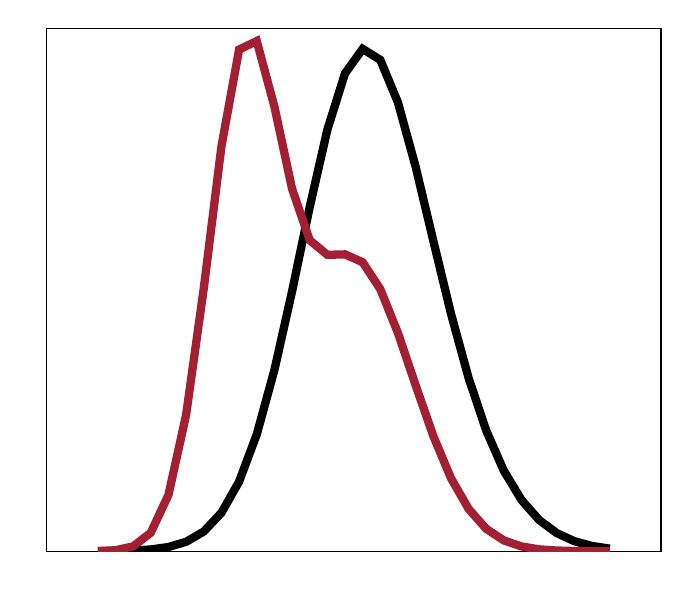
\begin{tikzpicture}
        \begin{axis}[-,domain=-3:4,scale =
          .4,xticklabels={,,},yticklabels={,,},ymin=0,ymax=.9,width=600pt, no
          marks,xticklabel style={major tick length=0pt},samples=30]
          \addplot[line width=3pt] {\gauss{1}{1}+\gauss{.5}{.8}};
          \addplot[line width=3pt,color=MITred] {\gauss{-1}{.5}+\gauss{.5}{.8}};
        \end{axis}
      \end{tikzpicture}
      \vspace{-1.5cm}
    \end{tabular}
  };
\node[state,
  below of=MODEL,
  node distance = 6.5cm,
  xshift = -3cm,
  anchor=west](SAMPLESPlots)
  {
    \begin{tabular}{l|c|c}
      {} &\textbf{Mean} & \textbf{Samples}\\
      \hline
      \rotatebox{90}{\textbf{\hspace{1.25cm}Prior}} &
      \includegraphics[scale=.125]{\figurepath/prmean.png} &
      \includegraphics[scale=.125]{\figurepath/prsample8.png}
      \includegraphics[scale=.125]{\figurepath/prsample10.png}
      \includegraphics[scale=.125]{\figurepath/prsample9.png}\\
      \hline
      \rotatebox{90}{\hspace{.55cm}\textcolor{MITred}{\textbf{Posterior}}}
                                                          &
      \includegraphics[scale=.125]{\figurepath/map.png} &
      \includegraphics[scale=.125]{\figurepath/postsample1.png}
      \includegraphics[scale=.125]{\figurepath/postsample100.png}
      \includegraphics[scale=.125]{\figurepath/postsample200.png}\\
    \end{tabular}
  };
\node[state,
  above of = SAMPLESPlots,
  node distance = 7.5cm,
  xshift = 8.5cm,
  anchor = east](TRUEPlots)
  {
    \begin{tabular}{|c|}
      \textbf{Truth}\\
      \includegraphics[scale=.13, trim=0 0 200 0, clip]{\figurepath/truth.png}
    \end{tabular}
  };

% draw the paths and and print some Text below/above the graph
\path
  (Input)        edge[line width=2pt] (MODEL)
  (MODEL)        edge[line width=2pt] (QoI)
  (DATA)         edge[line width=2pt] (BAYES)
  (BAYES)        edge[line width=2pt, bend left=5, color=MITred]
  node[other, anchor=north,rotate=0,xshift=0mm]{posterior} (Input)
  (Input)        edge[line width=2pt, bend left=10] node[other, anchor=south,rotate=0]{prior} (BAYES)
  (MODEL)        edge[line width=2pt, bend right=20, ->]
  node[other, anchor=west,xshift=0.1cm,yshift=-.2cm]{$\pi_\text{like}(\mathbf{d}|
  \textcolor{red}{\mathbf{m}}) = \pi_\text{noise}(\mathbf{F}(\textcolor{red}{\mathbf{m}}) - \mathbf{d})$}
  (BAYES);
\end{tikzpicture}
\end{document}
